\pagestyle{plain}

\setlength{\textheight}{7.0in}
\setlength{\parskip}{1.5ex plus 0.2ex minus 0.2ex}
\setlength{\parindent}{0cm}
\titlespacing{\section}{0pt}{10pt}{0pt}

\section{Om ordbogens tilblivelse -- pri la ekesto de la vortaro}
{\selectlanguage{danish}\itshape
de Jacob Nordfalk}

{\selectlanguage{esperanto}\frenchspacing
Inter 2007 kaj 2009 mia familio kaj mi lo\^gis en Nepalo, unu el la
landoj kun la plej malri\^caj lo\^gantaroj de la mondo (la\u{u} malneta
nacia produkto po lo\^ganto). Kvankam la esperantistoj tie elturni\^gas
diversmaniere, mi ofte pripensis \^cu ne eblus iel doni al ili
enspezojn: Pro la malaltaj salajroj kaj vivkostoj, nepalaj
esperantistoj povus fari laboron por Esperanto, kiu estus tro
longda\u{u}ra por fari libertempe en nia parto de la mondo. Mi sukcesis
kolekti monon por tiaj projektoj (interalie por fari la filmojn pri
Mejzi la Muso) inter esperantistoj de pli ri\^caj landoj.}

{\selectlanguage{esperanto}\frenchspacing
Tiam mi a\u{u}dis de Kim Henriksen pri la vortara projekto de Preben
Bagger: Li havis tre ellaboritan vortaron, sed nur kiel mane skribitan
manuskripton, kiun estus tro koste entajpi en Danio -- kaj venis la
ideo trovi nepalan esperantiston por fari tiun laboron. Mi telefonis al
Preben kaj proponis la ideon kaj ni interkonsentis elprovi \^cu la ideo
funkcios.

Tiel interkonsentite, mi vizitis Preben Bagger somere 2009 kaj skanis
lian manuskripton. La literojn A-F li anta\u{u}e enkomputiligis, sed la
dosiero perdi\^gis -- li nenion plu havis enkomputile, nur surpapere.
Dum tago mi enskanis \^cion haveblan: 71 pa\^goj kun la literoj A-F kun
mane skribitaj korektoj, A-E sen korektoj (por transformi al
kruddokumento per optika signorekono), kaj G-T kiel mane skribita
manuskripto de 731 pa\^goj. }

\begin{center}
	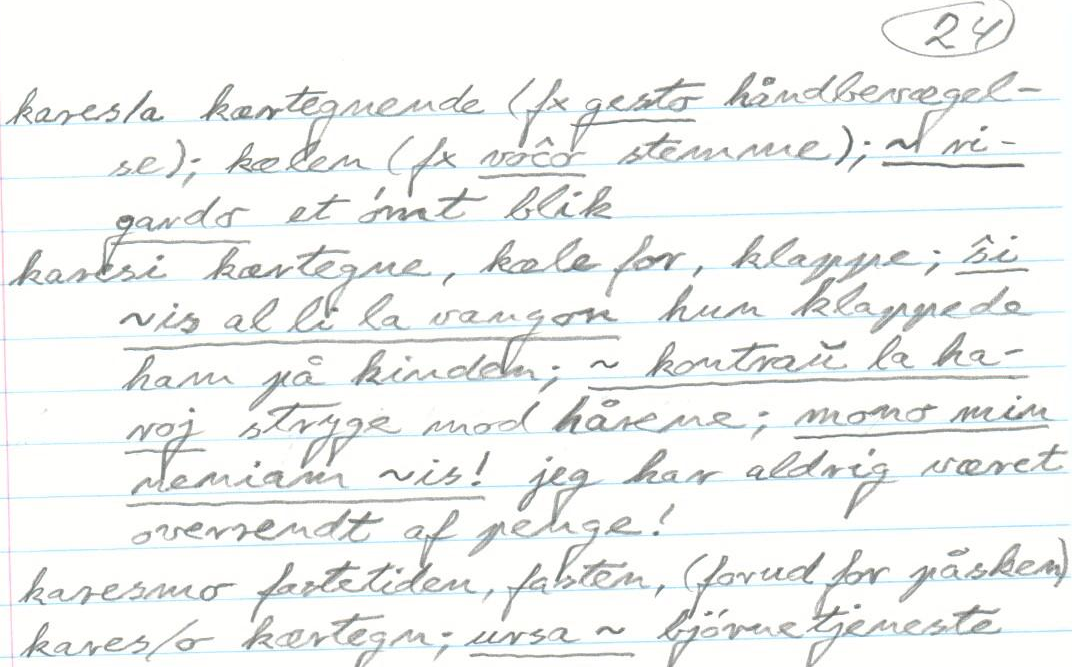
\includegraphics[width=10.5cm]{origino.png}
	
	{\selectlanguage{esperanto}\frenchspacing\itshape
	Parto de unu el la 731 pa\^goj de la mane skribita manuskripto}
	
\end{center}


{\selectlanguage{esperanto}\frenchspacing
Reveninte al Nepalo mi prezentis la manuskripton kaj la ideon al nepalaj
esperantistoj, kaj juna virino, Alinka Pokhrel, pretis preni la taskon,
kaj dum la sekva jaro \^si uzis pli ol 1500~laborhorojn por entajpi kaj
kontroli la 800 pa\^gojn, kontra\u{u} normala Nepala studenta salajro.
Danke al DEFA (Dana Esperanta Fervojista Asocio) ni ricevis malnovan
komputilon kun dana literumkontrolilo, kiu povis helpi \^sin literumi
preska\u{u} \^ciun danan vorton \^guste, kvankam \^si ne parolis la
danan:}


\begin{center}
\fbox{
\begin{minipage}{10.5cm}
\begin{alltt}
Pg. 24
\newline
\newline
kares/a k{\ae}rtegnende (fx \underline{gesto} h{\aa}ndbev{\ae}gelse); k{\ae}len (fx
\underline{voc\^{}o} stemme); \underline{\T{}rigardo} et {\o}mt blik
\newline
\newline
karesi\ \  k{\ae}rtegne, k{\ae}le for, klappe; \underline{s\^{}i \T{}is al li\ \ la vangon}
hun klappeda ham p{\aa}\ \ kinden; \underline{\T{} kontrau\^{} la karoj} stryge mod
h{\aa}rene; \underline{mono min neniam \T{}is!} jeg har aldrig v{\ae}ret overrendt
af penge!
\newline
\newline
karesmo\ \ \ \ \ \ \ \ \ \ fastetiden,  fasten, (forud for p{\aa}sken)
\newline
\newline
kares/o k{\ae}rtegn; \underline{ursa\T{}} bj{\o}rnetjenste
\end{alltt}
\end{minipage}
}

{\itshape La sama parto, post entajpo de Alinka}
\end{center}





{\selectlanguage{esperanto}\frenchspacing
\^Ciuj dosieroj de tiuj unuaj fazoj estas el\^suteblaj de la adreso:\\
\textit{http://javabog.dk/esperanto/dana\_vortaro\_bagger/}}

{\selectlanguage{esperanto}\frenchspacing
Dum 2010 mi ser\^cis kunlaborantojn kiuj volus helpi kontroli kaj
kompletigi la entajpitan manuskripton kaj trovis Jytte Sunek{\ae}r kaj
Peter Weide. Dum tri jaroj ni laboradis en nia libera tempo pri la
perfektigo de la manuskripto. Ni provis konservi la originalajn ideojn
kaj stilon de Preben, anka\u{u} en la literoj T, U, \u{U}, V kaj Z,
kiujn Peter Weide lerte ellaboris (parto de litero T estis jam farita, kaj Jytte finfaris \^gin).}

{\selectlanguage{esperanto}\frenchspacing
Preben transdonis \^ciujn rajtojn pri la materialo al ni, .... kaj ni
nun \^satus pludoni tiujn rajtojn al vi:}

\section{Permesilo -- copyright}
{\selectlanguage{danish}
Undertegnende Preben Bagger overdrager hermed Jacob Nordfalk samtlige
rettigheder over det til ham tidligere udleverede materiale til
ESPERANTO-DANSK ordbog, og jeg fraskriver mig hermed alle rettigheder
til det n{\ae}vnte materiale.}

{\selectlanguage{danish}
Vi, Peter Weide, Jytte Sunek{\ae}r og Jacob Nordfalk, tillader hermed
enhver digital og fysisk brug, {\ae}ndring og reproduktion af ordbogen,
s{\aa} l{\ae}nge der er en angivelse af kilden.}

{\selectlanguage{danish}
Vi har arbejdet med st{\o}rste omhu. Alligevel vil l{\ae}seren finde
fejl. Vi vil v{\ae}re taknemmelige, hvis man informerer os, s{\aa} vi
kan rette fejlene. Forslag til nye ord er selvf{\o}lgelig ogs{\aa}
velkomne. Vi beder om at anvendelser i trykte ordb{\o}ger venter, til
denne udgave er udsolgt.}

{\selectlanguage{esperanto}\frenchspacing
\textit{Tiu \^ci verko estas komuna hava\^{\j}o; vi rajtas uzi la verkon
}\foreignlanguage{danish}{\textit{kia}}\textit{ \^gi estas, komerce
a\u{u} nekomerce, plibonigi, \^san\^gi, adapti. Kion ajn. La sola
kondi\^co estas ke vi menci}\textit{u}\textit{ la fonton.}}

{\selectlanguage{esperanto}\frenchspacing
Ni laboris la\u{u}eble atenteme. Tamen eraroj trovi\^gos. Ni kun danko
akceptas informojn pri ili kaj la\u{u}eble rapide korektos ilin.
Memkompreneble anka\u{u} proponoj pri aldono de novaj vortoj estas
bonvenaj. Dankon al la ekspresa helpo de Jens S. Larsen kaj Regin Larsen tuj anta\u{u} la presado.}

{\selectlanguage{esperanto}\frenchspacing
Ni petas (ne postulas, sed petas) ke viaj uzoj ne rekte malgrandigu la
vendadon de tiu \^ci eldono, \^gis \^gi el\^cerpi\^gos.}


{\selectlanguage{danish}
Jacob Nordfalk, Peter Weide kaj Jytte Sunek{\ae}r}

{\selectlanguage{danish}
Valby, junio 2014.}


\begin{center}
	
\includegraphics[width=3cm]{permisilo.png}
\end{center}

\begin{center}
{\selectlanguage{esperanto}\frenchspacing\itshape
\^Ci tiu verko estas disponebla la\u{u} la permesilo\\
Krea Komuna\^{\j}o Atribuite 4.0 Tutmonda.\\
Vi povas legi la tutan permesilon \^ce:\\
http://creativecommons.org/licenses/by/4.0/deed.eo}
\end{center}
